%-----------------------------------------------------------------------
% A comparison of the mx FD solvers
% --------------------------------------------
\documentclass[11pt]{article} 

\input documentationPageSize.tex
%% \pagestyle{empty}

% \addtolength{\oddsidemargin}{-.975in}
% \addtolength {\textwidth} {2.0in}

% \addtolength{\topmargin}{-1.0in}
% \addtolength {\textheight} {1.5in}

% \voffset=-1.25truein
% \hoffset=-1.truein
% \setlength{\textwidth}{6.75in}      % page width
% \setlength{\textheight}{9.5in}    % page height

\input homeHenshaw

\newcommand{\url}[1]{}% ******** Remove URL's from bibtex entries ********
% \newcommand{\citeCount}[1]{}% for citation counts papers for WDH citations

\input{pstricks}\input{pst-node}
\input{colours}

% or use the epsfig package if you prefer to use the old commands
\usepackage{epsfig}
\usepackage{calc}
\input clipFig.tex

% The amssymb package provides various useful mathematical symbols
\usepackage{amsmath}
\usepackage{amssymb}

\newcommand{\Largebf}{\sffamily\bfseries\Large}
\newcommand{\largebf}{\sffamily\bfseries\large}
\newcommand{\largess}{\sffamily\large}
\newcommand{\Largess}{\sffamily\Large}
\newcommand{\bfss}{\sffamily\bfseries}
\newcommand{\smallss}{\sffamily\small}

\newcommand{\beq}{\begin{equation}}
\newcommand{\eeq}{\end{equation}}
\newcommand{\Omegav}{\boldsymbol{\Omega}}
\newcommand{\omegav}{\boldsymbol{\omega}}

\input wdhDefinitions.tex
\newcommand{\mbar}{\bar{m}}
\newcommand{\Rbar}{\bar{R}}
\newcommand{\Ru}{R_u}         % universal gas constant
% \newcommand{\grad}{\nabla}
\newcommand{\Div}{\grad\cdot}
\newcommand{\tauv}{\boldsymbol{\tau}}
\newcommand{\sigmav}{\boldsymbol{\sigma}}
\newcommand{\sumi}{\sum_{i=1}^n}


\newcommand{\Gc}{{\mathcal G}}
\newcommand{\Pc}{{\mathcal P}}
\newcommand{\Hc}{{\mathcal H}}
\newcommand{\Ec}{{\mathcal E}}
\newcommand{\Ic}{{\mathcal I}}

\newcommand{\eps}{\epsilon}
\newcommand{\kappav}{{\boldsymbol\kappa}}

\newcommand{\dt}{{\Delta t}}
% \newcommand{\figWidth}{5cm}

\newcommand{\ee}{{\rm e}}
\newcommand{\maxNorm}[1]{\|#1\|_\infty} 
\newcommand{\curl}{\grad\times}

\newcommand{\bogus}[1]{}

\newcommand{\tableFont}{\footnotesize}
% \usepackage{verbatim}
% \usepackage{moreverb}
% \usepackage{graphics}    
% \usepackage{epsfig}    
% \usepackage{fancybox}    

% tell TeX that is ok to have more floats/tables at the top, bottom and total
\setcounter{bottomnumber}{9} % default 2
\setcounter{topnumber}{9}    % default 1 
\setcounter{totalnumber}{15}  % default 3
\renewcommand{\textfraction}{.001}  % default .2

\begin{document}
 
\title{A Comparison of Different Methods for Solving Maxwell's Equations}

\author{
Bill Henshaw \\
% \  \\
% Centre for Applied Scientific Computing, \\
% Lawrence Livermore National Laboratory, \\
% henshaw@llnl.gov 
}
 
\maketitle

\tableofcontents

\section{Introduction}

These notes describe results of a comparison between some different approaches to 
solving the time domain Maxwell equations.
%
The three methods considered here are implemented in the cgmx solver~\cite{max2006b}:
\begin{itemize}
  \item A second-order finite-difference method that solves the second-order system on overlapping grids (CGFD2).
  \item A fourth-order finite-difference method that solves the second-order system on overlapping grids (CGFD4).
  \item The classical second-order Yee or FDTD scheme~\cite{Taflove2000,Yee66} (Yee).
\end{itemize}

We consider the following examples for comparison,
\begin{itemize}
  \item A plane wave traveling through free space.
  \item A PEC cylinder in two dimensions.
  \item A dielectric cylinder in two dimensions.
  \item A plane material interface in three-dimensions.
  \item A dielectric sphere. 
\end{itemize}

\clearpage
% -----------------------------------------------------------
\newcommand{\tol}{\tau}
\subsection{Order of Accuracy and Points Per Wavelength}


Suppose that we which to compute a solution to Maxwell's equations with a relative error
of $\tol$. 

The number of grid points we need depends on the wavelength $\lambda$ of the wave, the number 
of periods $T$ over which we wish to compute and the order of accuracy $q$ of our discrete
method.

Define $N_q$ to be the number of points per wavelength that we need. Then by an analysis of the
truncation error~\cite{GustafssonKreissOliger95} one can show that
\begin{align*}
  \text{Points-per-wavelength} &= N_q \approx C_q \left( {T \over \tol}\right)^{1/q}
\end{align*}
for some constants $C_q$ that are independent of $q$ and $\tol$.


\begin{table}[hbt]
\begin{center}
\begin{tabular}{|l|c|c|c|}\hline
                    & 2nd order   & 4th order    & 6th order   \\
Tolerance           & $N_2$         & $N_4$          & $N_6$          \\ \hline
$\tol=10^{-1}$ & $20 T^{1/2}$  & $7 T^{1/4}$    &  $5 T^{1/6}$   \\
$\tol=10^{-2}$ & $64 T^{1/2}$  &$13 T^{1/4}$    &  $8 T^{1/6}$   \\\hline
\end{tabular}
\end{center}
\caption{ Points per wavelength to obtain a relative error tolerance $\tol$ for a time interval of $T$ periods.}
\label{tab:PPW}
\end{table}


In $d$-space dimensions we will need $O(N_q^d)$ grid points and the computational work will be $O(N_q^{d+1})$
since we need to take $O(N_q)$ time steps. Assume that the $q-$order method requires $M_q$ work units
per grid point. The ratio of the total work for the 2nd-order method, $W_2$ to work for the 
4th order method, $W_4$ is 
\begin{align*}
  {W_2 \over W_4 } & 
    \approx {M_2 \over M_4} \left({C_2 \over C_4}\right)^{d+1}   \left( {T \over \tol}\right)^{(d+1)/4}  .
\end{align*}

We see that the second-order method becomes increasingly expensive
compared to the fourth order method as we require more accuracy for long time itervals.

% Given that ${C_2 \over C_4}\approx 3$ and ${M_2 \over M_4}$ is approximately $1/3$ to $1/5$ ?  


\clearpage
%-------------------------------------------------------------------------------------------------
\section{A plane wave in free space}\label{sec:planeWave}

In this example we propagate a plane wave in free space. The computational domain is a box, $[0,1]^3$
and the plane wave is $\Ev = \av \cos(2\pi(\kv\cdot\xv - \omega t) )$ with
$\av=( 1, -.5, -1)$ and $\kv=(3,2,2)$.

Figure~\ref{fig:planeWaveConvergenceRatesMaxNorm} 
and tables~\ref{table:planeWaveBoxYeeOrder2max}-\ref{table:planeWaveBoxNFDTDOrder4max} show
results for the Yee, CGFD2 and CGFD4 schemes. The Yee and CGFD2 schemes have
computed convergence rates of close to 2. The rate for CGFD4 is close to 4 and as expected the errors are
significantly smaller, especially on the finer grids. Also note that $\grad\cdot\Ev$ is not zero
for the Yee scheme but remains constant for all time steps.

Table~\ref{tab:planeWaveCPU} gives some CPU times for the different codes. The Yee scheme
is about 4 times slower than CGFD2 and $1.5$ times slower than CGFD4 for this case. There are two reasons
why it is slower. The first reason is that the Yee scheme is implemented for variable coefficients
(i.e. $\epsilon=\epsilon(\xv)$ and $\mu=\mu(\xv)$). The second reason is that the Yee scheme 
solves for six unknowns in $\Ev$ and $\Hv$ compared to the three unknowns $\Ev$ for the CGFD schemes.


\begin{figure}[hbt]
\begin{center}\small
\includegraphics[width=8cm]{planeWave/planeWaveConvergenceRatesMaxNorm.eps}
%
\caption{Convergence rates for a plane wave in free space. The maximum errors are given as the grid is refined.}
\label{fig:planeWaveConvergenceRatesMaxNorm}
\end{center}
\end{figure}

\begin{table}[hbt]
\begin{center}
\begin{tabular}{|l|c|c|c|}\hline
Method  & cpu (s/step) & cpu (s/step/pt) &  Yee/method   \\ \hline
Yee     &   2.76e-01   &   4.49e-07      &    1     \\
CGFD2   &   6.47e-02   &   1.05e-07      &    4.3    \\
CGFD4   &   1.88e-01   &   3.07e-07      &    1.5   \\ \hline
\end{tabular}
\end{center}
\caption{ CPU times for a plane wave in free space, box, $80^3$ grid points.}\label{tab:planeWaveCPU}
\end{table}


% *********** Yee 
%               ---------Maxwell Summary------- 
%                        Wed Jun 10 19:05:05 2009
%                Grid:   box80.order2 
%   ==== numberOfStepsTaken =      154, grids=1, gridpts =614125, interp pts=0, processors=1 ==== 
%   ==== memory per-proc: [min=135.93,ave=135.93,max=135.93](Mb), max-recorded=201.488 (Mb), total=135.93 (Mb)
%    Timings:         (ave-sec/proc:)   seconds    sec/step   sec/step/pt     %     [max-s/proc] [min-s/proc]
% total time..........................  4.47e+01    2.90e-01    4.73e-07   100.000   4.471e+01   4.471e+01
% setup and initialize................  9.66e-02    6.27e-04    1.02e-09     0.216   9.660e-02   9.660e-02
% initial conditions..................  4.70e-01    3.05e-03    4.97e-09     1.051   4.698e-01   4.698e-01
% advance.............................  4.25e+01    2.76e-01    4.49e-07    95.055   4.250e+01   4.250e+01
%    (advOpt).........................  4.25e+01    2.76e-01    4.49e-07    95.047   4.250e+01   4.250e+01
%   update ghost (parallel)...........  1.63e-03    1.06e-05    1.72e-11     0.004   1.631e-03   1.631e-03
% get errors..........................  7.23e-01    4.70e-03    7.65e-09     1.617   7.231e-01   7.231e-01
% compute dt..........................  1.36e-04    8.83e-07    1.44e-12     0.000   1.360e-04   1.360e-04
% plotting............................  8.84e-01    5.74e-03    9.34e-09     1.976   8.835e-01   8.835e-01
% waiting (not counted)...............  5.09e-04    3.31e-06    5.38e-12     0.001   5.090e-04   5.090e-04
% 
%               ---------Maxwell Summary------- 
%                        Thu Jun 11 13:24:33 2009
%                Grid:   box80.order2 
%   ==== numberOfStepsTaken =      154, grids=1, gridpts =614125, interp pts=0, processors=1 ==== 
%   ==== memory per-proc: [min=87.4961,ave=87.4961,max=87.4961](Mb), max-recorded=0 (Mb), total=87.4961 (Mb)
%    Timings:         (ave-sec/proc:)   seconds    sec/step   sec/step/pt     %     [max-s/proc] [min-s/proc]
% total time..........................  1.30e+01    8.44e-02    1.38e-07   100.000   1.300e+01   1.300e+01
% setup and initialize................  6.22e-02    4.04e-04    6.57e-10     0.478   6.218e-02   6.218e-02
% initial conditions..................  5.52e-01    3.59e-03    5.84e-09     4.248   5.525e-01   5.525e-01
% advance.............................  9.97e+00    6.47e-02    1.05e-07    76.646   9.967e+00   9.967e+00
%   advance rectangular grids.........  2.98e+00    1.93e-02    3.15e-08    22.905   2.979e+00   2.979e+00
%    (advOpt).........................  2.97e+00    1.93e-02    3.14e-08    22.841   2.970e+00   2.970e+00
%   add dissipation...................  2.95e+00    1.91e-02    3.11e-08    22.649   2.945e+00   2.945e+00
%   boundary conditions...............  4.03e+00    2.62e-02    4.26e-08    31.011   4.033e+00   4.033e+00
%   interface bc......................  2.40e-05    1.56e-07    2.54e-13     0.000   2.400e-05   2.400e-05
% get errors..........................  1.62e+00    1.05e-02    1.71e-08    12.427   1.616e+00   1.616e+00
% compute dt..........................  9.80e-05    6.36e-07    1.04e-12     0.001   9.800e-05   9.800e-05
% plotting............................  8.01e-01    5.20e-03    8.47e-09     6.161   8.012e-01   8.012e-01
% 
%               ---------Maxwell Summary------- 
%                        Thu Jun 11 13:26:22 2009
%                Grid:   box80.order4 
%   ==== numberOfStepsTaken =      154, grids=1, gridpts =614125, interp pts=0, processors=1 ==== 
%   ==== memory per-proc: [min=87.5234,ave=87.5234,max=87.5234](Mb), max-recorded=0 (Mb), total=87.5234 (Mb)
%    Timings:         (ave-sec/proc:)   seconds    sec/step   sec/step/pt     %     [max-s/proc] [min-s/proc]
% total time..........................  3.24e+01    2.10e-01    3.42e-07   100.000   3.236e+01   3.236e+01
% setup and initialize................  6.22e-02    4.04e-04    6.57e-10     0.192   6.216e-02   6.216e-02
% initial conditions..................  5.47e-01    3.55e-03    5.78e-09     1.690   5.469e-01   5.469e-01
% advance.............................  2.90e+01    1.88e-01    3.07e-07    89.650   2.901e+01   2.901e+01
%   advance rectangular grids.........  1.79e+01    1.16e-01    1.89e-07    55.326   1.790e+01   1.790e+01
%    (advOpt).........................  1.79e+01    1.16e-01    1.89e-07    55.300   1.789e+01   1.789e+01
%   add dissipation...................  5.04e+00    3.27e-02    5.33e-08    15.578   5.041e+00   5.041e+00
%   boundary conditions...............  6.05e+00    3.93e-02    6.40e-08    18.712   6.055e+00   6.055e+00
%   interface bc......................  2.70e-05    1.75e-07    2.85e-13     0.000   2.700e-05   2.700e-05
% get errors..........................  1.92e+00    1.25e-02    2.03e-08     5.932   1.919e+00   1.919e+00
% compute dt..........................  9.70e-05    6.30e-07    1.03e-12     0.000   9.700e-05   9.700e-05
% plotting............................  8.15e-01    5.30e-03    8.62e-09     2.520   8.154e-01   8.154e-01
% 
\clearpage
\input planeWave/planeWaveBoxYeeOrder2maxNormConvTable.tex

\input planeWave/planeWaveBoxNFDTDOrder2maxNormConvTable.tex

\input planeWave/planeWaveBoxNFDTDOrder4maxNormConvTable.tex


\clearpage
%-------------------------------------------------------------------------------------------------
\section{Scattering from a dielectric cylinder}\label{sec:dielectricCylinder}

In this example we consider the scattering of a plane wave from a
two-dimensional cylinder. 
A glass cylinder, $\epsilon=2.25$, radius $r=.4$ is embedded in free space $\epsilon=1$. 


Tables~\ref{table:dielectricCylYeeOrder2max}-\ref{table:dielectricCylNFDTDOrder4max}
give convergence rates for the maximum errors. The incident field is $\Ev = \av \cos(2\pi(\kv\cdot\xv - \omega t) )$ with
$\av=( 0, 1)$ and $\kv=(1.25,0)$. The wavelength of the incident field is equal to $d=.8$, the diameter of the cylinder.
The errors in the Yee scheme are large at the interface since the normal component of the
electric field is discontinuous and the grid is not aligned with the interface.
As a result the maximum errors for the Yee scheme do not decrease as the grid is refined. 
On the other hand, CGFD2 converges at second-order
and CGFD4 converges at fourth-order for this problem. These schemes use a grid that is aligned with the interface.

Figure~\ref{fig:dielectricCylConvergenceRatesMaxNorm} and tables~\ref{table:dielectricCylYeeOrder2L1}-\ref{table:dielectricCylNFDTDOrder4L1} 
give convergence rates for the average error ($L_1$ norm).
In the $L_1$ norm the Yee scheme does converge at first order. CGFD2 and CGFD4 converge
at 2nd and 4th order respectively.

\begin{figure}[hbt]
\begin{center}\small
\includegraphics[width=8cm]{dielectricCyl/dielectricCylConvergenceRatesMaxNorm.eps}
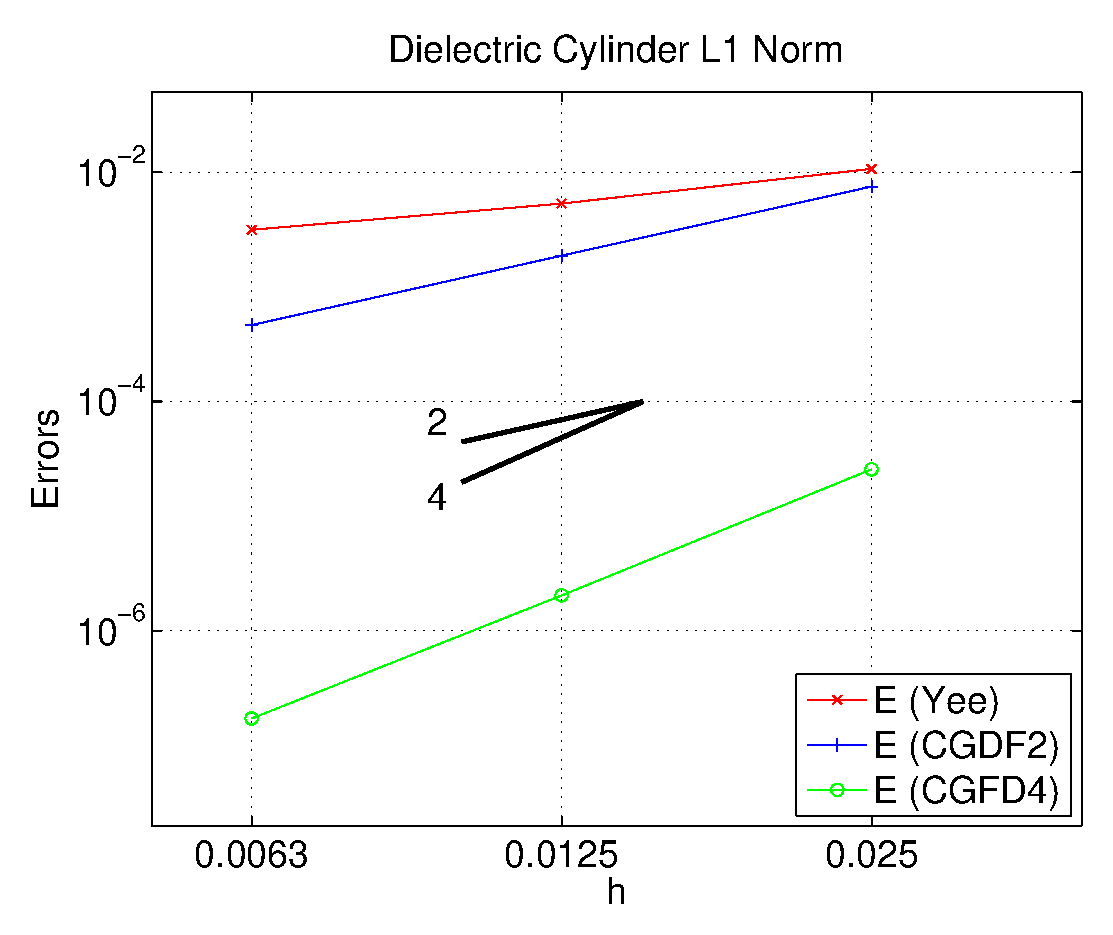
\includegraphics[width=8cm]{dielectricCyl/dielectricCylConvergenceRatesL1Norm.eps}
%
\caption{Convergence rates for the dielectric cylinder.  
  The maximum (left) and $L_1$-norm (right) errors are given as the grid is refined.}
\label{fig:dielectricCylConvergenceRatesMaxNorm}
\end{center}
\end{figure}

CPU times are given in table~\ref{tab:dielectricCylCPU}. The number of grid points for the 
Yee scheme is slightly less than the other cases. The Yee scheme is about 10\% slower than
CGFD2 but 4 times faster than CGFD4. About 50\% of the time for CGFD4 is spent in iterating
to solve the interface conditions. This could be reduced to about 10\% by implementing a better algorithm.

\begin{table}[hbt]
\begin{center}
\begin{tabular}{|l|c|c|c|c|c|}\hline
Method  & grid-pts  & cpu (s)      & cpu (s/step) & cpu (s/step/pt) &  Yee/method (cpu) \\ \hline
Yee     &  1.1e5    &   5.2        &  2.06e-02    &  1.95e-07     &     1    \\
CGFD2   &  1.3e5    &    4.7       &  1.51e-02    &  1.16e-07     &     1.1   \\
CGFD4   &  1.3e5    &   21.7       &  7.82e-02    &  5.95e-07     &     .24  \\ \hline
\end{tabular}
\end{center}
\caption{ CPU times for scattering from a dielectric cylinder.}\label{tab:dielectricCylCPU}
\end{table}


\clearpage
\input dielectricCyl/dielectricCylYeeOrder2maxNormConvTable

\input dielectricCyl/dielectricCylCGFD2Order2maxNormConvTable

\input dielectricCyl/dielectricCylCGFD4Order4maxNormConvTable
% \input dielectricCyl/dielectricCylCGFD4Order4maxNormConvTableDissOrder8

\clearpage
\input dielectricCyl/dielectricCylYeeOrder2L1NormConvTable
\input dielectricCyl/dielectricCylCGFD2Order2L1NormConvTable.tex
\input dielectricCyl/dielectricCylCGFD4Order4L1NormConvTable.tex


\input dielectricCylFig

%               ---------Maxwell Summary------- 
%                        Fri Jun 12 09:06:13 2009
%                Grid:   bigSquareSize1f16 
%   ==== numberOfStepsTaken =      254, grids=1, gridpts =105625, interp pts=0, processors=1 ==== 
%   ==== memory per-proc: [min=30.4023,ave=30.4023,max=30.4023](Mb), max-recorded=36.0078 (Mb), total=30.4023 (Mb)
%    Timings:         (ave-sec/proc:)   seconds    sec/step   sec/step/pt     %     [max-s/proc] [min-s/proc]
% total time..........................  1.12e+01    4.39e-02    4.16e-07   100.000   1.115e+01   1.115e+01
% setup and initialize................  1.38e-02    5.43e-05    5.14e-10     0.124   1.380e-02   1.380e-02
% initial conditions..................  5.84e+00    2.30e-02    2.18e-07    52.354   5.838e+00   5.838e+00
% advance.............................  5.23e+00    2.06e-02    1.95e-07    46.861   5.225e+00   5.225e+00
%    (advOpt).........................  5.22e+00    2.06e-02    1.95e-07    46.816   5.220e+00   5.220e+00
%   update ghost (parallel)...........  2.13e-03    8.39e-06    7.94e-11     0.019   2.131e-03   2.131e-03
% get errors..........................  1.68e-02    6.62e-05    6.27e-10     0.151   1.681e-02   1.681e-02
% compute dt..........................  2.15e-04    8.46e-07    8.01e-12     0.002   2.150e-04   2.150e-04
% plotting............................  4.90e-02    1.93e-04    1.83e-09     0.440   4.904e-02   4.904e-02
% waiting (not counted)...............  3.61e-04    1.42e-06    1.35e-11     0.003   3.610e-04   3.610e-04
%               ---------Maxwell Summary------- 
%                        Thu Jun 11 14:12:47 2009
%                Grid:   innerOutere8.order2 
%   ==== numberOfStepsTaken =      315, grids=4, gridpts =130149, interp pts=1824, processors=1 ==== 
%   ==== memory per-proc: [min=39.8711,ave=39.8711,max=39.8711](Mb), max-recorded=39.8047 (Mb), total=39.8711 (Mb)
%    Timings:         (ave-sec/proc:)   seconds    sec/step   sec/step/pt     %     [max-s/proc] [min-s/proc]
% total time..........................  6.29e+00    2.00e-02    1.53e-07   100.000   6.291e+00   6.291e+00
% setup and initialize................  8.65e-02    2.75e-04    2.11e-09     1.375   8.648e-02   8.648e-02
% initial conditions..................  1.35e+00    4.30e-03    3.30e-08    21.536   1.355e+00   1.355e+00
% advance.............................  4.74e+00    1.51e-02    1.16e-07    75.411   4.744e+00   4.744e+00
%   advance rectangular grids.........  3.61e+00    1.14e-02    8.80e-08    57.330   3.607e+00   3.607e+00
%   advance curvilinear grids.........  3.49e-01    1.11e-03    8.52e-09     5.551   3.492e-01   3.492e-01
%    (advOpt).........................  3.56e+00    1.13e-02    8.69e-08    56.607   3.561e+00   3.561e+00
%   add dissipation...................  2.17e+00    6.89e-03    5.29e-08    34.497   2.170e+00   2.170e+00
%   boundary conditions...............  1.70e-01    5.38e-04    4.14e-09     2.695   1.695e-01   1.695e-01
%   interface bc......................  3.92e-01    1.24e-03    9.55e-09     6.226   3.917e-01   3.917e-01
%   interpolation.....................  1.40e-01    4.45e-04    3.42e-09     2.227   1.401e-01   1.401e-01
% get errors..........................  1.01e-01    3.21e-04    2.46e-09     1.605   1.010e-01   1.010e-01
% compute dt..........................  9.53e-04    3.03e-06    2.32e-11     0.015   9.530e-04   9.530e-04
% plotting............................  6.38e-02    2.03e-04    1.56e-09     1.015   6.384e-02   6.384e-02
%               ---------Maxwell Summary------- 
%                        Fri Jun 12 20:34:16 2009
%                Grid:   innerOutere8.order4 
%   ==== numberOfStepsTaken =      278, grids=4, gridpts =131421, interp pts=3648, processors=1 ==== 
%   ==== memory per-proc: [min=41.9766,ave=41.9766,max=41.9766](Mb), max-recorded=41.8516 (Mb), total=41.9766 (Mb)
%    Timings:         (ave-sec/proc:)   seconds    sec/step   sec/step/pt     %     [max-s/proc] [min-s/proc]
% total time..........................  2.33e+01    8.40e-02    6.39e-07   100.000   2.334e+01   2.334e+01
% setup and initialize................  8.24e-02    2.96e-04    2.26e-09     0.353   8.239e-02   8.239e-02
% initial conditions..................  1.37e+00    4.94e-03    3.76e-08     5.884   1.373e+00   1.373e+00
% advance.............................  2.17e+01    7.82e-02    5.95e-07    93.158   2.174e+01   2.174e+01
%   advance rectangular grids.........  2.17e+00    7.79e-03    5.93e-08     9.281   2.166e+00   2.166e+00
%   advance curvilinear grids.........  2.63e+00    9.45e-03    7.19e-08    11.260   2.628e+00   2.628e+00
%    (advOpt).........................  2.20e+00    7.91e-03    6.02e-08     9.427   2.200e+00   2.200e+00
%   add dissipation...................  1.28e+00    4.60e-03    3.50e-08     5.482   1.280e+00   1.280e+00
%   boundary conditions...............  1.71e-01    6.16e-04    4.68e-09     0.733   1.712e-01   1.712e-01
%   interface bc......................  1.51e+01    5.43e-02    4.13e-07    64.630   1.509e+01   1.509e+01
%   interpolation.....................  3.21e-01    1.16e-03    8.79e-09     1.376   3.212e-01   3.212e-01
% get errors..........................  1.28e-01    4.60e-04    3.50e-09     0.548   1.279e-01   1.279e-01
% compute dt..........................  1.44e-03    5.18e-06    3.94e-11     0.006   1.441e-03   1.441e-03
% plotting............................  6.59e-02    2.37e-04    1.80e-09     0.282   6.593e-02   6.593e-02

\clearpage
%-------------------------------------------------------------------------------------------------
\section{A plane material interface}\label{sec:planeMaterialInterface}

We consider a plane wave that hits a plane material interface in three-dimensions.
We start by writing down the solution for the general case in 3D. 
Note that the coefficients of reflection and refraction depend on the polarization of
the incident field (see Balanis~\cite{Balanis89}).

Consider an incident plane wave $\Ev = \av e^{i (\kv\cdot\xv - \omega t)}$ traveling in direction $\kv$ that
hits a plane material interface with normal $\nv$.
The {\em plane of incidence} is the plane defined by the two vectors $\kv$ and $\nv$ that
passes through some point $\xv_0$ on the interface (we assume $\nv\cdot\kv \ne 0$). 
Define the two vectors
\begin{align}
  \qv &= \frac{\nv \times \kv}{\vert \nv \times \kv \vert}, \qquad\text{(unit normal to the plane of incidence)},\\
  \gv &= \frac{\qv \times \kv}{\vert \qv \times \kv \vert}, \qquad\text{(unit vector in the plane of incidence, normal to $\kv$)},
\end{align}
which define a basis for the plane orthogonal to $\kv$. The incident field can thus be decomposed into
components in the direction of $\qv$ and $\gv$,
\begin{align}
  \av &= E_\perp \qv + E_\parallel \gv, \\
   E_\perp &= \av\cdot\qv,  \qquad\text{(coefficient of the perpendicular polarization)}\\
   E_\parallel &= \av\cdot\gv,  \qquad\text{(coefficient of the parallel polarization)} .
\end{align}
The wave vectors of the reflected and transmitted waves are defined by 
\begin{align}
  \kv^r &= \kv - 2 (\kv\cdot\nv)\nv , \qquad\text{(reflected wave vectors)}, \\
  \kv^t &= \kv + ( k_n^t - \kv\cdot\nv)\nv, , \qquad\text{(transmitted wave vectors)},\\
  k_t &= \sqrt{ \kv\cdot\kv - (\nv\cdot\kv)^2 } , \\
  k_n &= \sqrt{ (c_1/c_2)^2 \kv\cdot\kv  - k_t^2 }
\end{align}
The coefficients of reflection and refraction for components perpendicular and parallel to the plane of incidence are
(these follow from the tangential components of the field being continuous and $[ \epsilon \nv\cdot\Ev]=0$), 
\begin{align}
   R_\perp &= { \eta_2\cos(\theta_i) - \eta_1 \cos(\theta_t) \over \eta_2\cos(\theta_i) + \eta_1 \cos(\theta_t) } \\
   T_\perp &= 1 + R_\perp\\
   R_\parallel &= { -\eta_1\cos(\theta_i) + \eta_2 \cos(\theta_t) \over \eta_1\cos(\theta_i) + \eta_2 \cos(\theta_t) } \\
   T_\parallel &= 1 + R_\parallel\\
   \cos\theta_i &= \kv\cdot\nv/\vert \kv \vert, \qquad\text{(angle of incidence)}, \\
   \eta_m & = \sqrt{\frac{\mu_m}{\epsilon_m}} , \qquad\text{(impedance)}, \\
   \vert \kv \vert \sin\theta_i &= \vert \kv^t \vert \sin\theta_t, \qquad\text{(Snell's law)} \\
   \theta^r &= \theta^i 
\end{align}
where $\mu_1$, $\epsilon_1$ define the incident state and $\mu_2$, $\epsilon_2$ define the material state.
The solution can thus be written as
\begin{alignat}{3}
   \Ev(\xv,t) &= \Ev_i  + \Ev_r , \qquad&&\text{for $\nv\cdot(\xv-\xv_0) < 0$} , \\
   \Ev(\xv,t) &= \Ev_t          , \qquad&&\text{for $\nv\cdot(\xv-\xv_0) > 0$} , 
\end{alignat}
where
\begin{align}
   \Ev_i &= \Big[ E_\perp \qv + E_\parallel \gv \Big] \exp(i(\kv\cdot\xv - \omega t)), \\
   \Ev_r &= \Big[ R_\perp E_\perp \qv + R_\parallel E_\parallel \hv \Big] \exp(i(\kv^r\cdot\xv - \omega t)), \\
   \Ev_t &= \Big[ T_\perp E_\perp \qv + T_\parallel E_\parallel \mv \Big] \exp(i(\kv^t\cdot\xv - \omega t)), 
\end{align}
and vectors $\hv$ and $\mv$ are 
\begin{align}
  \hv &= \frac{\qv \times \kv^r}{\vert \qv \times \kv^r \vert},\\
  \mv &= \frac{\qv \times \kv^t}{\vert \qv \times \kv^t \vert} 
\end{align}



{\bf To finish: } provide results...

For the Yee scheme we consider an interface that is parallel to the grid and one that is not parallel. 



\clearpage
%-------------------------------------------------------------------------------------------------
\section{Scattering from a dielectric sphere}\label{sec:dielectricSphere}

In this example we consider the scattering of a plane wave from a
sphere.
A glass sphere of radius $r=1$, $\epsilon=2.25$, is embedded in free space $\epsilon=1$. 
The incident plane wave is $\Ev = \av \cos(2\pi(\kv\cdot\xv - \omega t) )$ with
$\av=( 0, 1., 0)$ and $\kv=(k_x,0,0)$.

Table~\ref{fig:dielectricSphereConvergenceRatesMaxNorm} compares the max-norm and $L_1$ norm errors
at $t=1$ for $k_x=1$. 

\begin{figure}[hbt]
\begin{center}\small
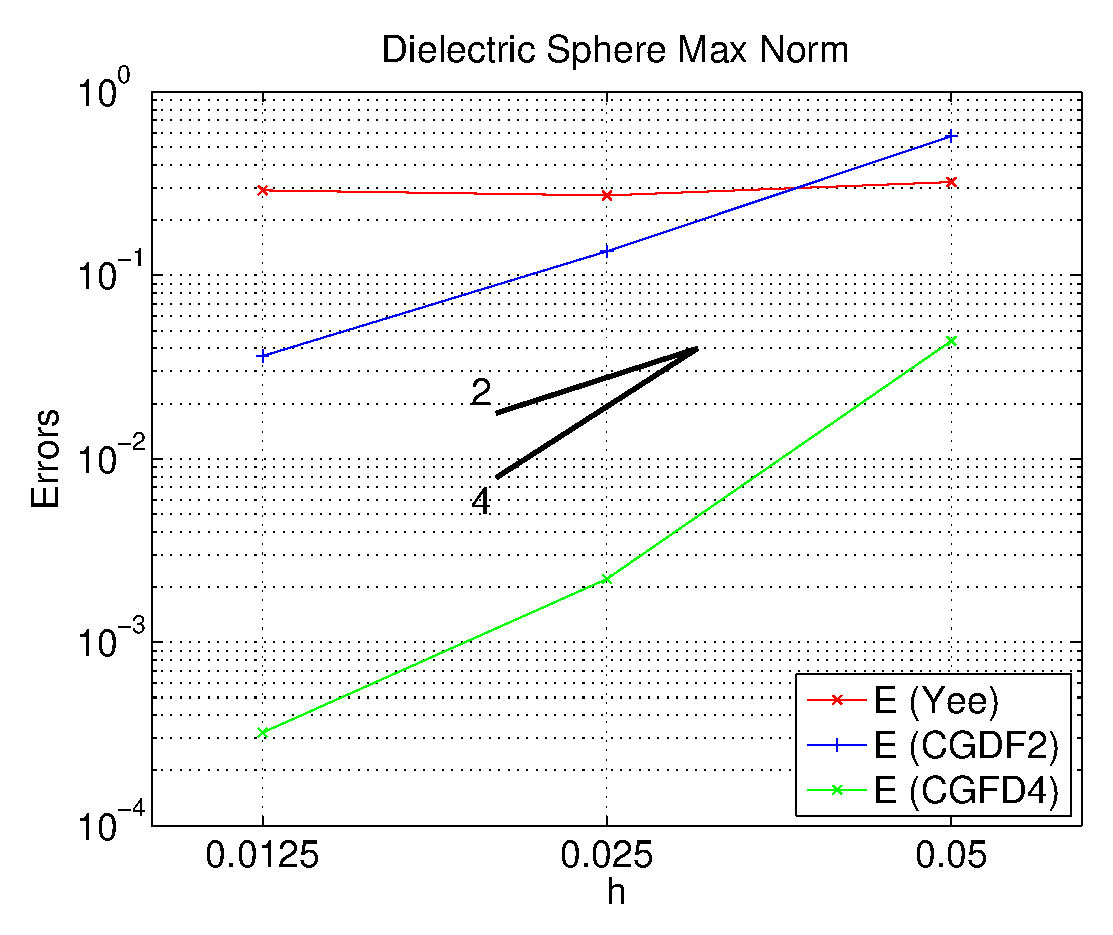
\includegraphics[width=8cm]{dielectricSphere/dielectricSphereConvergenceRatesMaxNorm.eps}
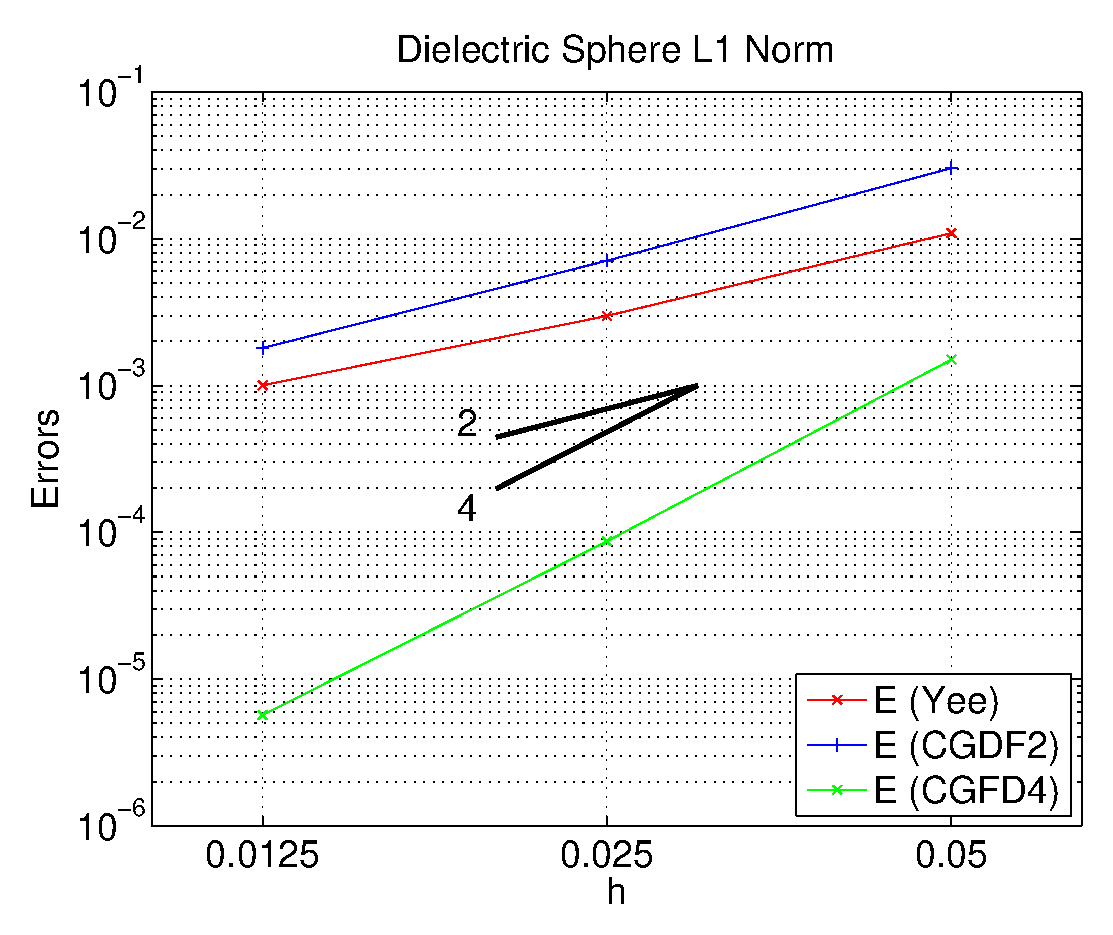
\includegraphics[width=8cm]{dielectricSphere/dielectricSphereConvergenceRatesL1Norm.eps}
%
\caption{Convergence rates for the dielectric sphere.
  The maximum (left) and $L_1$-norm (right) errors are given as the grid is refined. }
\label{fig:dielectricSphereConvergenceRatesMaxNorm}
\end{center}
\end{figure}

CPU times are given in table~\ref{tab:dielectricSphereCPU} {\bf finish me...}

\begin{table}[hbt]
\begin{center}
\begin{tabular}{|l|c|c|c|c|c|}\hline
Method  & grid-pts  & cpu (s)      & cpu (s/step) & cpu (s/step/pt) &  Yee/method (cpu) \\ \hline
Yee     &  3.43281e+07    &              &              &               &     1    \\
CGFD2   &  3.81586e+07    &              &              &               &           \\
CGFD4   &  3.81586e+07    &              &              &               &          \\ \hline
\end{tabular}
\end{center}
\caption{ CPU times for scattering from a dielectric sphere.}\label{tab:dielectricSphereCPU}
\end{table}

Figure~\ref{fig:scatDielectricSphereCGFD4Fig} shows the computed solution at $t=1.$.

\input dielectricSphereFig


\clearpage
\bibliography{\homeHenshaw/papers/common/henshawPapers}
\bibliographystyle{siam}

\end{document}


% ----------------------------------------------------------------------------------------------------------



